% Jeg tror det er tre spørsmål som kan besvares her:
% 1. Hvor mye enklere/bedre er det å utvikle apps med Kvik microservices?
% 2. Overhead/ improvement for enkelt-microservices. Dvs overhead for de som
% tilbyr noe mer en alternativet (container tilbyr enklere deployment men har en
% overhead på...), og improvement for de som optiamliserer noe (Kvik vs OpenCPU,
% eventuelt begge deler (caching for MsigDB reduserer query tid men har en
% storage overhead)
% 3. Performance analyse av MIxT. Hvor er det overheadene er for en query? Overhead for mange samtidige queries?
%
% Metodologi:
% 1. Kvik-MIxT vs 1000-R-linjer-MIxT? Og kanskje anektdoter som at container
% kunne flyttes til AWS. Eller noe helt annet.
% 2. En av de enklere web apps som er laget før. Eventuelt en benchmark app.
% 3. MIxT operasjoner.
%
We show the viability and need for Kvik by describing the MIxT application for
exploring and comparing transcriptional profiles from blood and tumor samples.
We describe its functionality, implementation 
% (uten fokus på Kvik)
and performance requirements.
%OG ANDRE VIKTIGE TING (SECURITY, ETC). 


\begin{figure}[h!]
\centering
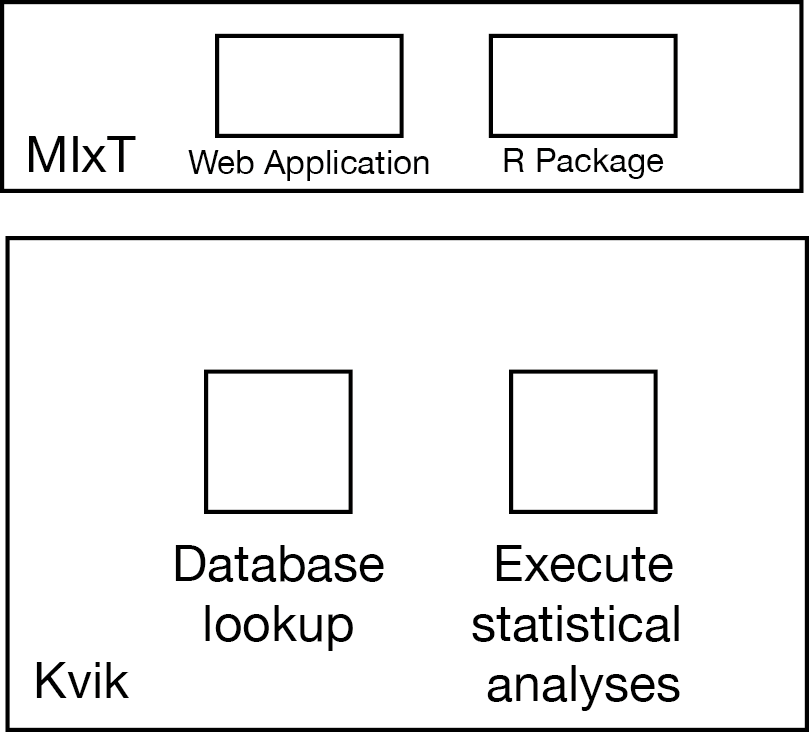
\includegraphics{figures/kvik-mixt.png}
\caption{An overview of the relationship between the MIxT application and Kvik.
MIxT contains a web application (online at \url{mixt-blood-tumor.bci.mcgill.ca})
and the R Package that provides analyses and data to the web application. Kvik
provides the services for running the statistical analyses from the R package,
and the database lookups found in the web application.} 
\label{kvik-mixt}
\end{figure} 


% Det kan godt være at vi bør flytte denne et sted, men her beskriver vi hvordan 
% MIxT-appen fungerer. 
\subsection*{WIP: Matched Interaction Across Tissues (MIxT)}

For the web application we defined six analysis tasks: 

\textbf{Explore co-expression relationships between genes}. Create an
interactive network visualization that visualizes each gene as a node and
significan co-expression relationship as an edge. 

\textbf{Explore co-expression gene sets in tumor and blood tissue}.
Visualize gene expression together with clinicopathological variables associated
with each module. Include results of gene set analyses that describe the
underlying biological functions of the modules. 

\textbf{Explore relationships between modules from each tissue.}
Visualize how modules from each tissue are related using two different
metrics, ranksum and gene overlap. Also enable subtype selection,
enabling users to investigate relationships within a particular subtype. 

\textbf{Explore relationships between clinical variables and modules.}
Visualize significant associations between module expression and
clinical variables.

\textbf{Explore association between user-submitted gene lists and computed
modules.} Allow users to upload own gene lists and have the application compute
modules which the gene list is enriched for. 

\textbf{Search for genes or gene lists of intrest.} Allow users to search
for specific genes or genelists of intrest and show what modules they are
associated with. 

% Vi kan godt kutte én av figurene under, f.eks c eller d som er veldig lik. 
\begin{figure*}[h!]
\centering
\caption{MIxT module overview page. The screenshot show the user interface for
exploring a single module. It consists of three panels. The top left panel
contains the gene expression heatmap. The top right panel contains a table of
the genes found in the module. The bottom panel contains the results of gene
overlap analyses from the module genes and known gene sets from MSigDB.}
%\caption{Screenshots of the user interface in four of the six analysis tasks.
%Note that we combine visualization frameworks for both JavaScript and R to
%generate the visualizations. Specifically, sigmajs (a,
%\protect\url{sigmajs.org}), ggplot2(b, \protect\url{ggplot2.org}), and D3 (c and
%d, \protect\url{d3js.org})}
%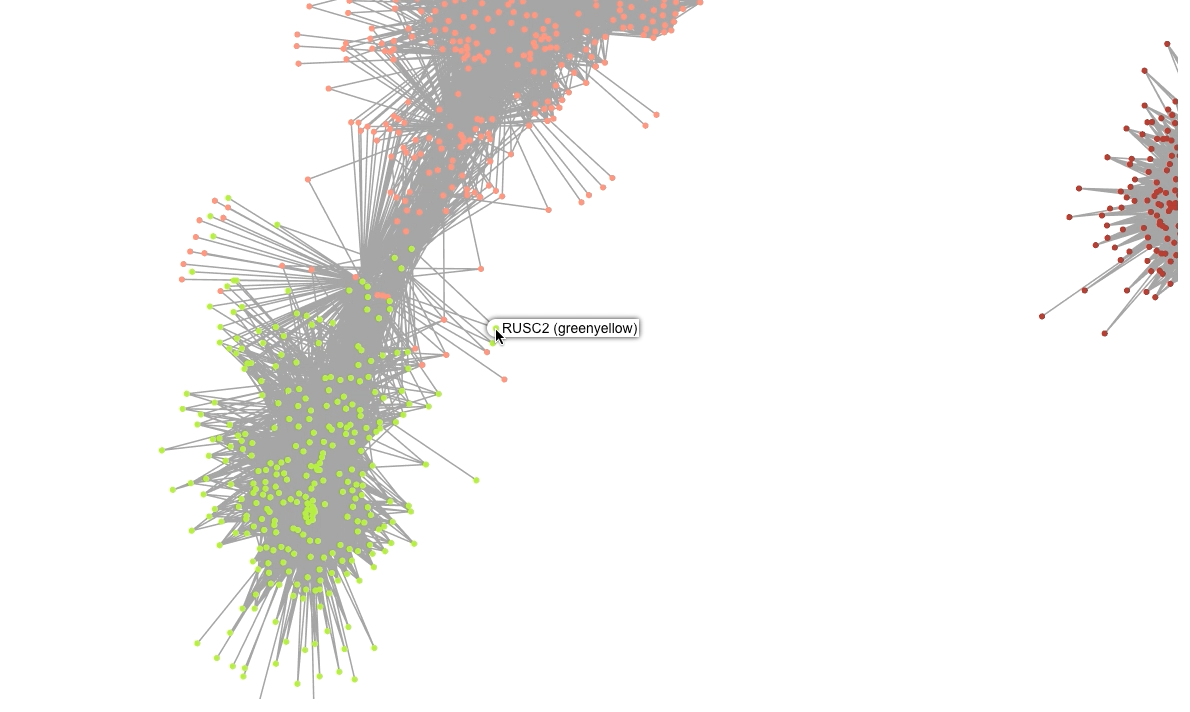
\includegraphics[width=2.7in]{figures/network.png} 
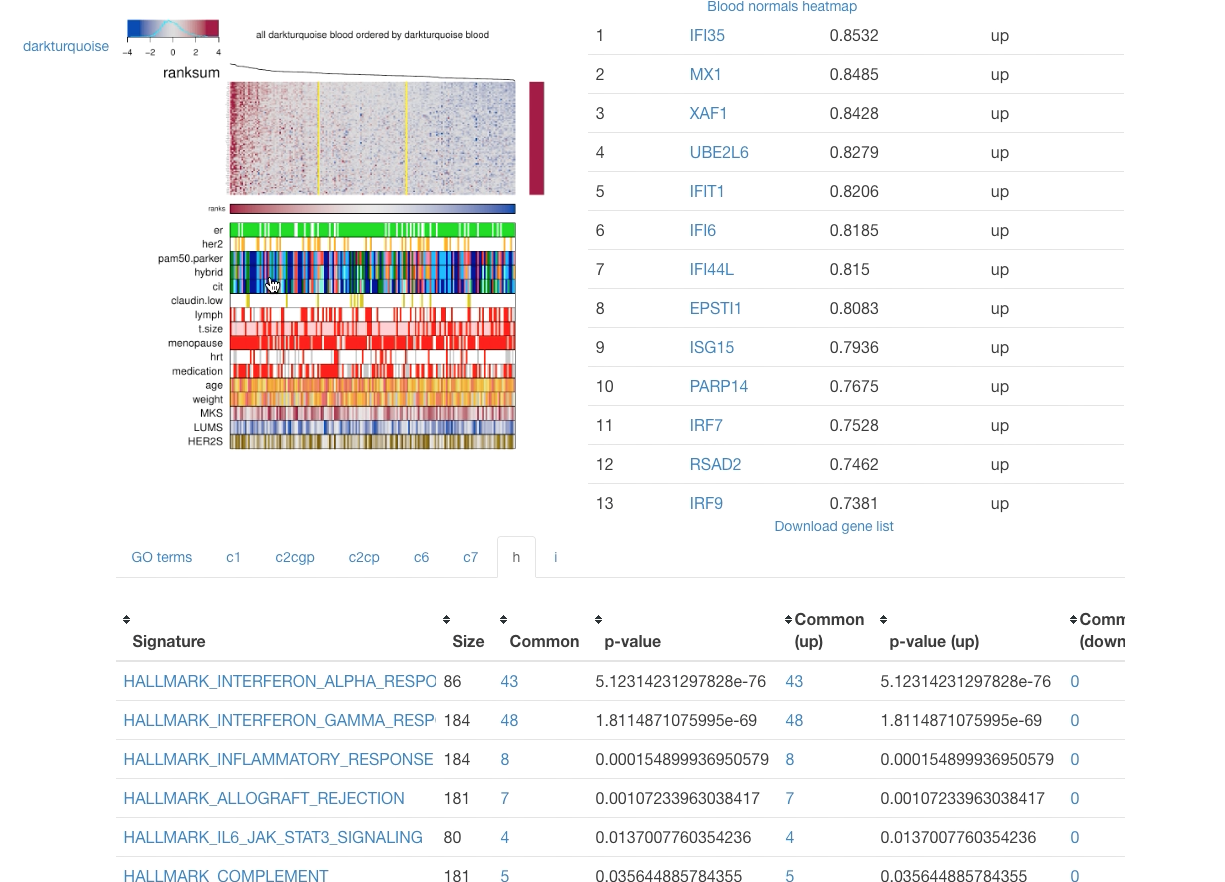
\includegraphics[width=0.8\textwidth]{figures/module.png}
% 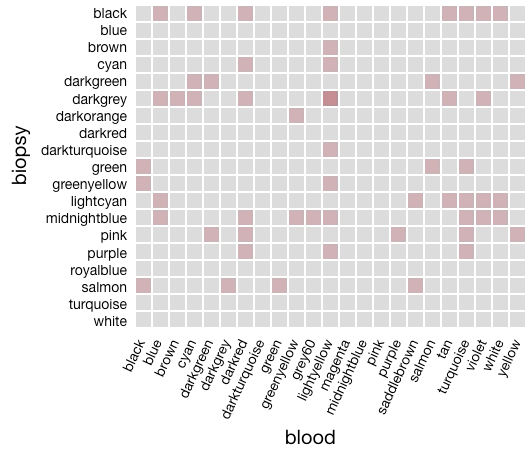
\includegraphics[width=2.5in]{figures/tissue-comp.png}
\label{fig_first_case}
\end{figure*} 

% \hfil
% \subfloat[A2: Module visualization.]{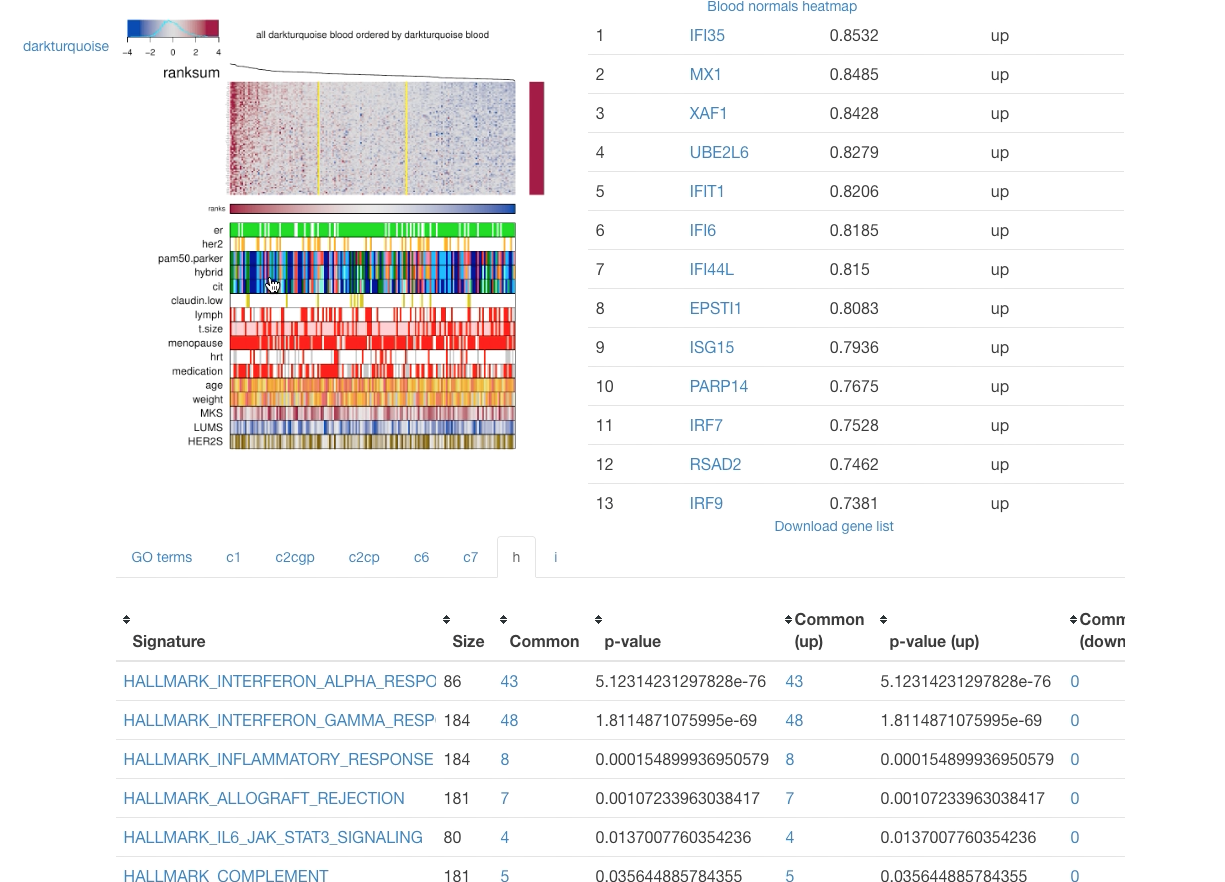
\includegraphics[width=2.5in]{figures/module.png}%
% \label{fig_second_case}}
% \hfil
% \centering
% \subfloat[A3: Visualization of ranksum.]{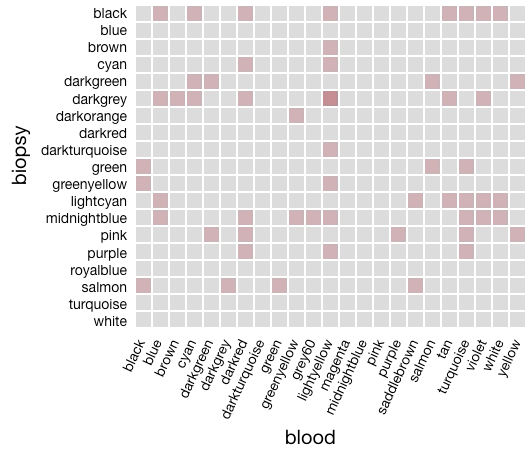
\includegraphics[width=2.5in]{figures/tissue-comp.png}%
% \label{fig_first_case}}
% \hfil
% \subfloat[A4: Visualization of significant clinical variable
% association]{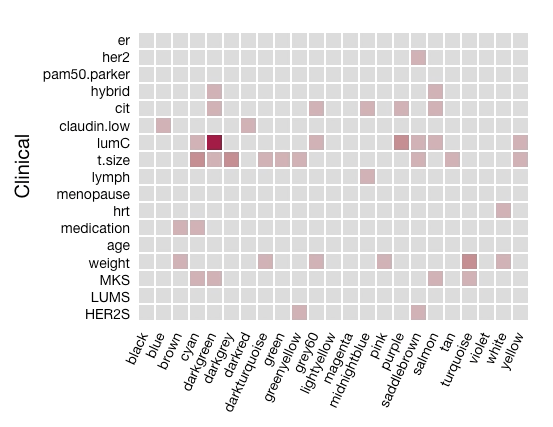
\includegraphics[width=2.8in]{figures/clinical-comp.png}%
% \label{fig_second_case}}
% \caption{Screenshots of the user interface in four of the six analysis tasks.
% Note that we combine visualization frameworks for both JavaScript and R to
% generate the visualizations. Specifically, sigmajs (a,
% \protect\url{sigmajs.org}), ggplot2(b, \protect\url{ggplot2.org}), and D3 (c and
% d, \protect\url{d3js.org})} 
% \label{fig_sim}
% \end{figure*}


\subsubsection*{WIP: MIxT design and Implementation}
The MIxT application is designed as a modern application consisting of multiple
services that together provide an interactive web application. By composing an
application of a set of services we can substitute parts of the application
without re-writing the entire application. This type of architectural style is
called a microservices architecture and is popular in 'web-scale' systems. For
example if we want to use OpenCPU to interface with data analysis we can do so
by simply exchanging the Kvik R service with OpenCPU. Both services communicate
over HTTP and their interface is the same. 

From our initial analyses we built
an R package with functions to provide data and analysis to the different
analysis tasks. Using this design it is possible to either explore the data
through the web site or a local R session. 

To explore the co-expression relationship between genes we use an interactive
graph visualization build with Sigmajs\footnote{\url{sigmajs.org}}. We have
built visualization for both tissues, with graph sizes of 2705 nodes and 90 348
edges for the blood network, and 2066 nodes and 50 563 edges for the biopsy
network. The sigmajs visualization library has functionality for generating a
layout for large networks, but we generate this layout server-side to reduce the
computational load on the client. To generate this layout we use the GGally
package\footnote{\url{cran.r-project.org/web/packages/GGally}}. 

We have built modules for each tissue, and to explore gene sets associated with
genes in these modules, we provide module overview pages that show gene
expression visualized together with clinicopathological variables and gene set
analyses that describe the underlying functions of the module. 

We have used different metrics to link the modules from each tissue, ranksum and
gene overlap. To visualize the associations we use the
d3\footnote{\url{d3js.org}} library to build an interactive heatmap
visualization. 

To allow users to explore the relationship between clinical variables and the
computed modules, we built an interctive heatmap visualization that visualizes
the association between different metrics and each module. 


